\chapter{Baze podataka u bioinformatici} % Main chapter title

\label{Baze} % For referencing 

Automatizacija bioloških i hemijskih analiza početkom 21. veka omogućila je
ubrzanu i paralelnu analizu velikog broja uzoraka. Ove tehnologije žargonski su
poznate kao \keyword{tehnologije velike propusnosti} \en{high throughput
technology }. Primera radi, tehnologije \keyword{sekvenciranja nove generacije}
\en{Next-Generation Sequencing} ili skraćeno \keyword{NGS} neprekidno napreduju
spuštajući cenu čitanja genoma i eksponencijalno povećavajući količinu dostupnih
sekvenci. Da bi se razumeo uticaj NGS tehnologije navodimo sledeći primer.
Od sveže sekvencionisanih nepoznatih genoma predviđaju se
potencijalni geni, od gena potencijalne proteinske sekvence.  Dobijene
proteinske sekvence mogu se dalje klasterovati u familije, automatski
anotirati, predviđati im se struktura, osobine itd.  Zatim, moguće je vršiti
analize za oktrivanje novih bioloških znanja. Povezanost između funkcije i
neuređenosti proteina je jedan primer biološkog znanja. 
Ovaj primer ilustruje dve bitne stvari:
\begin{enumerate}
  \item Eksponencijalni rast podataka uvodi bioinformatiku u oblast Big Data,
    posebno njene discipline poznate pod nazivom omike (na primer, genomike, proteomika itd.)
  % \item Informacije eksponencijalno rastu uvodeći čitavu oblast
  %   \keyword{omike}\footnote{termin objedinjuje gen\textbf{omiku}, proteomiku,
  %   transkriptomiku, glikomiku...} \en{omics}  u teritoriju \en{Big
  % Data} \parencite{Chen2017}.
  % (U našem radu pažljivo su odabrani podaci malog
  % obima kako bi se izbegao ovaj scenario i sve analize su urađene na klasičnom
  % kućnom računaru.)
  \item Velika povezanost između bioloških podataka.
\end{enumerate}

Povezanost podataka preslikava se na baze podataka. Većina baza je usko specijalizovana
za jedan tip informacije ili jedan organizam, ali zato sadrži reference ka
drugim (spoljnim) bazama, naučnim radovima ili  manje formalnim, ali
informativnim resursima (veb strane, vikipedija, itd...). Specijalne baze podataka kao
što je \uniprotkb, pored primarnog sadržaja održavaju i veliki broj referenci ka
drugim bazama podataka (tzv. dbxref \en{database cross reference}) pokušavajući
da međusobno povežu sve dostupne informacije. Konkrentno \uniprotkb (feb. 2018)
održava reference ka čak 164 različite baze
podataka\footnote{\url{www.uniprot.org/docs/dbxref}}.  Dakle, bioinformatika
kao disciplina podrazumeva da će analize biti vršene kombinacijom informacija
nekoliko različitih baza.  Zbog raznovrsnosti i svrhe prikupljenih informacija
postoji veliki broj kategorija\footnote{Baze podataka ne pripadaju ekskluzivno
samo jednoj kategoriji}(vrsta) baza. Na adresi \cite{dbSummary2015} autori Čen, Huang i Vu
kategorizovali su i prikazali novije, javno dostupne i visoko kvalitetne
proteinski orijentisane baze podataka (prikazana lista nije iscrpna) \parencite{Chen2017}.
Za temu ovog rada od značaja su naredne tri kategorije:

\begin{itemize}
  \item Baze sekvenci.\\ 
        Ove baze podataka sadrže sve poznate javno dostupne sekvence i kontrolišu dodeljivanje 
        identifikacionog broja sekvence.
    \begin{itemize}
      \item Proteinske sekvence: \uniprotkb
      \item DNK sekvence: EMBL-Bank, GenBank, DDBJ, ...
    \end{itemize}
  \item Baze strukture: DisProt, D2P2, MobiDB, PDB, ...
  \item Baze ontologija: Gene Ontology, Protein Ontology
\end{itemize}


\section{Ontologije gena}

\keyword{Ontologija Gena} \en{Gene Ontology} ili skraćeno \keyword{GO}, 
% predstavlja izračunato znanje o funkciji gena odnosno genskog
predstavlja znanje o funkciji gena odnosno genskog
produkta (protein, nekodirajuća RNK ili makromolekulskih kompleks)
\parencite{GO2016}.
GO baza sačinjena je iz dve komponente:
\begin{enumerate}
  \item \keyword{Ontologije gena}.
  \item \keyword{GO anotacije} tj. anotacije genskog produkta \keyword{GO terminom}. U našoj
    analizi anotacije su preuzete iz \swissprot baze podataka\footnote{Ali \swissprot koristi anotacije iz ontologije gena}.
\end{enumerate}

Ontologija gena definiše skup termina, takozvanih \keyword{GO termina}
\en{GO terms} i njihove međusobne relacije. GO termini predstavljaju biološke
termine (koncepte) koji opisuju funkciju. Ontologija gena sagledava funkciju
genskog produkta iz tri aspekta koji se u terminologiji ontologija nazivaju
imenski prostori \en{namespace}:
\begin{itemize}
  \item \keyword{Molekulska funkcija (MF)} je biohemijska aktivnost (uključujući
    specifično vezivanje za ligande\footnote{
      Ligand je supstanca koja formira kompleks sa biomolekulom u cilju izvršavanja biološke funkcije. TODO
    } ili strukture) genskog produkta.
  \item \keyword{Ćelijske komponente  (CC)} se odnosi na mesto u ćeliji gde je
    genski produkt aktivan.
  \item \keyword{Biološki procesi (BP)} se odnose na procese kome genski produkt
    doprinosi.
\end{itemize}

Inspirisani sličnošću prva tri sekvencirana eukariotska organizma, GO projekat
nastao je sa ciljem da  unifikuje biologiju pod jedan univerzum termina za opis
genskih proizvoda svih vrsta organizama \parencite{GO2000}.

Suštinu ontologije čine relacije između termina i pravila dedukcije koja se nad
njima mogu primenjivati. Osnovnu strukturu ontologije čini usmereni aciklički
graf \en{DAG} obrazovan roditeljskom vezom (relacijom) \keyword{is\_a}. Prateći
ovu relaciju termini jednog imenskog prostora na primer MF neće nikad preći u
druga dva CC i BP.  Ontologija stoga ima tri korena čvora MF, CC i BP
\parencite{go_struktura}. Primer strukture prikazan je na
Slici \ref{fig:kinase}.  Pored \keyword{is\_a} postoje dodatne relacije od kojih
su najčešće:

\begin{itemize}
  \item \keyword{part\_of}  - je deo  (ne znači da je uvek deo vezanog termina, relacija agregacije)
  \item \keyword{has\_part} - sadrži (deo uvek postoji, relacija kompozicije)
  \item \keyword{regulates} - pozitivna ili negativna regulacija
  \item \keyword{positvely\_regulates} - pozitivna regulacija  
    (\keyword{is\_a} termin koji reguliše)
  \item \keyword{negatively\_regulates} - negativna regulacija 
    (\keyword{is\_a} termin koji reguliše)
\end{itemize}

\begin{figure}[h!]
  \centering
  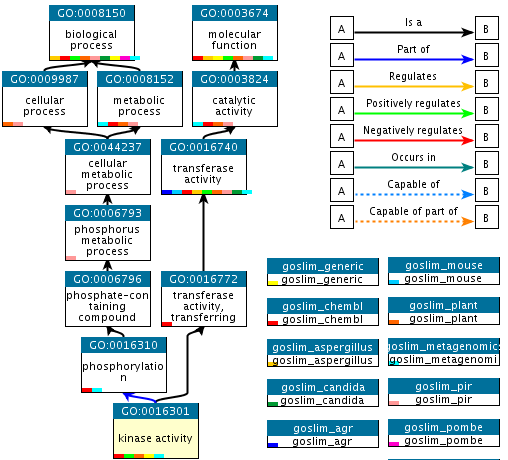
\includegraphics[width=0.8\linewidth]{img/kinase.png}
  \caption{Struktura ontologije\\ \footnotesize (preuzeto sa geneontology.org)}
  \label{fig:kinase}
\end{figure}

Vremenom se ontologija proširuje novim tipovima relacije koje su van okvira ovog rada.
Svaka veza (relacija) ima strogo definisana pravila kompozicije koja omogućavaju
automatsko rezonovanje. Na primer relacija \keyword{is\_a} ima svojstvo
tranzitivnosti \parencite{is_a} prikazano Slikom \ref{fig:is_a}:
\lstset{
  basicstyle=\ttfamily, mathescape,
  numbers=none
}

\begin{figure}[h!]
  \centering
\begin{lstlisting}
         A is_a    B  $\wedge$   B is_A C  $\implies$    A is_a    C           
         A part_of B  $\wedge$   B is_A C  $\implies$    A part_of C
\end{lstlisting}
\caption{Tranzitivnost relacije \keyword{is\_a}}
  \label{fig:is_a}
\end{figure}


Siže pravila rezonovanja prikazan je na Slici \ref{fig:relations}.

Jedan od najčešće korišćenih formata je  ravni \file{.obo} format a pored njega
su u upotrebi \file{RDF/XML} i \file{OWL} formati.  Poslednja dva formata
namenjena su automatskom rezonovanju unutar specijalizovanih softvera i upitnih
jezika (protégé, SPARQL, ...).

\begin{figure}[h!]
  \centering
  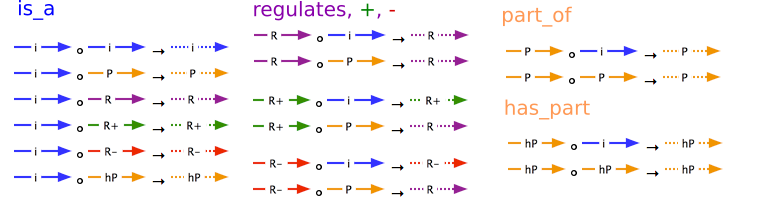
\includegraphics[width=1.0\linewidth]{relations.png}
  \caption{Pravila rezonovanja (isprekidane relacije su rezultat)}
  \label{fig:relations}
\end{figure}

GO termin može biti zastareo u kom slučaju se relacijom \keyword{replaced\_by}
pokazuje na noviji termin. Relacija \keyword{consider} ukazuju na
postojanje mogućih ekvivalentnih termina. Pored glavnog univerzuma postoje i
podskupovi\footnote{Uglavnom ovi podskupovi predstavljaju model organizme}
termina (GO slim) prikazani u donjem desnom delu Slike \ref{fig:kinase}.


\subsection{Molekulska funkcija}
TODO, treba proučiti \parencite{go_mf} možda nešto saznam o kvalitetu anotacija
u \swissprot bazi.



\section{UniProtKB/Swiss-Prot}
\label{svis-prot}

\keyword{\uniprot} skraćeno od \en{Universal Protein Resource} je konzorcijum
nastao 2002. izmedju tri organizacije: Evropski Bioinformatički
Institut (EBI), Švajcarski institut za Bioinformatiku (SIB) i Resurs
Proteinskih Informacija (PIR).  


\uniprot obuhvata nekoliko baza i podbaza sa striktno definisanim tokom
informacija Slika \ref{fig:uniprot_overview}. Od prikazanih najbitnija je
\keyword{\uniprotkb} \en{UniProt Knowledge Base} sačinjena od 2 podbaze.

\begin{figure}[h!]
  \centering
  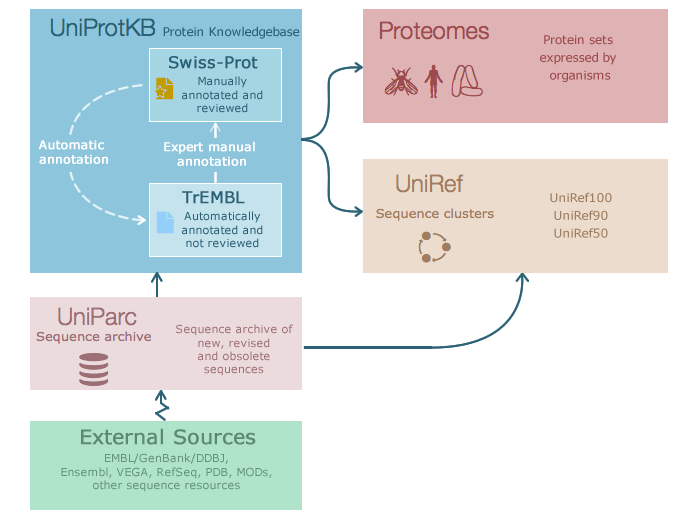
\includegraphics[width=0.8\linewidth]{uniprot_overview.png}
  \caption{Šematski prikaz povezanosti \uniprot baze\\ \footnotesize (preuzeto sa uniprot.com)}
  \label{fig:uniprot_overview}
\end{figure}


\begin{enumerate}
  \item \keyword{\swissprot}  sadrži visoko kvalitetne anotacije
    \keyword{ne redundantnih} (stavka\ref{red}) proteinskih sekvenci.
    Informacije o sekvenci su dobijene iz postojeće literature, a kompjuterski
    predviđene anotacije su ručno proverene. \swissprot kao baza postoji preko
    30 godina.

  \item \trembl \en{Translated EMBL} je nadskup \swissprot sekvenci 
    dobijen prevođenjem EMBL i drugih nukleinskih sekvenci. Automatskom
    računarskom analizom anotirane su i opisane ali zbog obimne količine ti
    rezultati još nisu ručno provereni.  Ove sekvence su redundantne i njihova
    obimnost posledica je masovne primene NGS tehnologija. U februaru 2018. god
    \trembl sadržao je 107 627 435 sekvenci što je oko 200 puta više u
    poređenju sa 556 568 ručno proverenih \swissprot sekvenci. Sve nove
    sekvence prvo ulaze u sastav \trembl da bi ručnom proverom napredovale u
    \swissprot što se ogleda na Slici \ref{fig:uniprot_overview}.
\end{enumerate}





Distribucije \swissprot baze dostupne su u nekoliko tekstualnih formata: ravna
datoteka \en{flat file}, XML, RDF/XML.  Ravni tekstualni format zbog
standardizacije prati EMBL-Bank\parencite{embl} ravni format
\parencite{svisprot2003}. Unos u bazu se zove \keyword{slog} \en{record} i
sadrži sve informacije vezane za jedan protein.  Jedan slog predstavljen u
formatu ravne datoteke ilustrovan je uporšćenim prikazom  na Slici \ref{fig:slog}.
Ključne osobine slogova i \swissprot baze podataka su:

\lstset{ 
  basicstyle=\footnotesize\ttfamily,        % the size of the fonts that are used for the code
  captionpos=b,                    % sets the caption-position to bottom
  commentstyle=\color{mygreen},    % comment style
  deletekeywords={...},            % if you want to delete keywords from the given language
  escapeinside={\%*}{*)},          % if you want to add LaTeX within your code
  extendedchars=true,              % does not work with UTF-8
  keywordstyle=\color{blue},       % keyword styli
  % language=Octave,                 % the language of the code
  morekeywords={ID, AC, PE, KW, GO, SQ}, % if you want to add more keywords to the set
  numbers=left,                    % where to put the line-numbers; 
  numbersep=5pt,                   % how far the line-numbers are from the code
  numberstyle=\color{mygray}, % the style that is used for the line-numbers
  % rulecolor=\color{black},         % if not set, the frame-color may be changed on line-breaks within not-black text (e.g. comments (green here))
  showstringspaces=false,          % underline spaces within strings only
}

\begin{figure}[h!]
  \centering

\begin{lstlisting}
ID   ACSA_DROME              Reviewed;         670 AA.  | ime sloga, info
AC   Q9VP61; Q24226; Q8IH30; Q9VP60;                    | identifikacija
DT   19-SEP-2003, integrated into UniProtKB/Swiss-Prot. | ulazak u Svis-Prot
DT   01-MAY-2000, sequence version 1.                   | ulazak u TrEMBL
DT   25-OCT-2017, entry version 116.                    | poslednje 
                                                          osvezavanje sloga
\end{lstlisting}
\begin{lstlisting}[firstnumber=7,   basicstyle=\footnotesize\ttfamily\color{gray}]
DE   RecName: Full=Acetyl-coenzyme A synthetase;        |
DE            EC=6.2.1.1;                               |
DE   AltName: Full=Acetyl-CoA synthetase;               |
DE            Short=ACS;                                |
GN   Name=AcCoAS; ORFNames=CG9390;                      |
OS   Drosophila melanogaster (Fruit fly).               | Taksonomija
OC   Eukaryota; Metazoa; Ecdysozoa; Arthropoda; Hexap...|
OC   Pterygota; Neoptera; Holometabola; Diptera; Brac...|
OC   Ephydroidea; Drosophilidae; Drosophila; Sophopho...|
OX   NCBI_TaxID=7227 {ECO:0000312|EMBL:AAL90278.1};     |
                                                        
RN   [1] {ECO:0000305}                                  | Prva referenca
RP   NUCLEOTIDE SEQUENCE (ISOFORM B).                   | 
RA   Russell S.R., Heimbeck G.M., Carpenter A.T., Ash...| Autori
RT   "A Drosophila melanogaster acetyl-CoA-synthetase...| Naslov
RL   Submitted (NOV-1994) to the EMBL/GenBank/DDBJ da...|
RN   [2]                                                | Druga referenca              
...                                                     
CC   -!- FUNCTION: Activates acetate so that it can b...| Komentari
CC       synthesis or for energy generation.            |
CC       {ECO:0000250|UniProtKB:Q9NR19}.                |
CC   -!- CATALYTIC ACTIVITY: ATP + acetate + CoA = AM...|
...                                                     
\end{lstlisting}
\begin{lstlisting}[firstnumber=30]
DR   EMBL; Z46786; CAA86738.1; ALT_SEQ; mRNA.           | reference ka
DR   EMBL; AE014296; AAF51695.2; -; Genomic_DNA.        | drugim bazama 
...                                                     | (dbxref)
DR   ExpressionAtlas; Q9VP61; differential.             |
DR   Genevisible; Q9VP61; DM.                           |
DR   GO; GO:0005737; C:cytoplasm; IEA:UniProtKB-SubCell.| GO termin <----
DR   GO; GO:0003987; F:acetate-CoA ligase activity; I...| GO termin <----
...                                                     |
\end{lstlisting}
\begin{lstlisting}[firstnumber=38]
PE   2: Evidence at transcript level;
KW   Alternative splicing; ATP-binding; Complete proteome; Cytoplasm; 
KW   Ligase; Nucleotide-binding; Reference proteome.                  
FT   CHAIN         1    670       Acetyl-coenzyme A synthetase.
FT                                /FTId=PRO_0000208425.
FT   VAR_SEQ       1    146       Missing (in isoform B).
FT                                {ECO:0000303|PubMed:12537569}.
FT                                /FTId=VSP_008310.
FT   CONFLICT    227    227       C -> S (in Ref. 1; CAA86738).
FT                                {ECO:0000305}.
SQ   SEQUENCE   670 AA;  75960 MW;  CE24364755CDBFFC CRC64;
     MPAEKSIYDP NPAISQNAYI SSFEEYQKFY QESLDNPAEF WSRVAKQFHW ETPADQDKFL
...
     KKMVRERIGP FAMPDVIQNA PGLPKTRSGK IMRRVLRKIA VNDRNVGDTS TLADEQIVEQ
     LFANRPVEAK
//  <--- oznacava kraj sloga
\end{lstlisting}
\caption{Uprošćen primer sloga, preuzet iz ravne datoteke \file{uniprot\_sport.data} \footnotesize (preuzeto sa FTP servera \cite{sprot})  }
\label{fig:slog}
\end{figure}


\begin{enumerate}
  \item Ime sloga \keyword{ID} \en{entery name} je mnemonički zapis koji kodira
    taksonomske informacije o genu i proteinu. ID je podložan promenama 
    i ne može se koristiti kao identifikator \parencite{www_uniprot}.
  \item Identifikacioni broj predstavlja \keyword{AC} \en{accession number}.
    Prvi u listi identifikatora naziva se \keyword{primarni} i služi da
    jednoznačno odredi slog. Ostatak identifikatora su tzv. \keyword{sekundarani AC} i
    nastaju iz dva moguća razloga \parencite{svisprot2003, www_uniprot}:
    \begin{itemize}
      \item Unifikacija postojećih proteina u jedan novi slog. 
      \item Specijalizacija jednog proteina u više različitih.
    \end{itemize}
    U oba slučaja stari (primarni) AC se zadržava kao sekundarni AC u novom slogu.

  \item Za razliku od \trembl, GO mapiranje za \swissprot sekvence određuju se ručno \parencite{www_uniprot}.

  \item \keyword{Ključne reči} \en{keywords} označene \keyword{KW} opisuju
    hijearhisku strukturu kontrolisanog vokabulara namenjenog opisivanju
    funkcije proteina. Postoji 10 kategorija ključnih reči od kojih je za naše
    istraživanje bitna "Molekulska funkcija"  \parencite{svisprot2003}.  Za
    razliku od GO čiji ideal je opis svih genskih produkta svih vrsta, termini
    ključnih reči prilagođeni su opisivanju sadržaja isključivo \swissprot
    proteina \parencite{www_uniprot}.

  \item Sekvenca \keyword{SQ} u slogu poznata je kao \keyword{kanonska}
    \en{canonical} sekvenca. Kanonska sekvenca predstavlja konsenzus sekvencu
    produkta (protein) gena jedne vrste organizma.  \keyword{FT} linije sadrži
    različite osobine kanonske sekvence uključujući i razlike u odnosu na
    izoforme\footnote{Izoforme su alternativni oblici sekvence nastali usled:
    alternativnog splajsovanja, upotrebe više promotera, alternativnih start
  kodona ili alternativnih okvira čitanja } sekvence.  U našoj analizi
  korišćena je isključivo kanonska sekvenca. Detaljan opis pravila za biranje
  kanonske sekvence može se naći na \parencite{www_uniprot}.

  \item
    \label{red}
    \swissprot je \keyword{minimalno redundantna} u smislu da svi proteini
    kodirani jednim genom, jedne vrste su predstavljeni jednim slogom. Sve
    izoforme su grupisane pod jedan slog i jednu kanonsku sekvencu \parencite{nonRedundant}.

  \item Postojnost proteina \keyword{PE} \en{Protein existance} opisuje stepen
    sigurnosti da protein postoji \ref{fig:PE}. Moguće vrednosti u rastućem poredku su:
    pronađeno na nivou proteina, pronađeno na nivou RNK, zaključeno iz homologije, predviđen i nesiguran. 

  \clearpage


  \item
    \swissprot takđe vrši predikcije neuređenih regiona:  koristeći \textit{DISOPRED2}
    and \textit{CLADIST} prediktor \parencite{Meng_c2017}\\ Međutim ove informacije
    postale su irelevantne pojavom baza neuređenja \\ \textit{MobiDB} i \textit{D2P2}.

  \item Zanimljiva zapažanja globalne statistike:
    \begin{itemize}
      \item Najzastupljenije sekvence su kraće od 500 aminokiselina.
      \item Postojnost oko $70\%$ proteina potvrđeno je homologijom.
      \item Zastupljeno je preko 1000 različitih organizama međutim
        većina \swissprot sekvenci pripada malom broju model organizama.
      \item Najviše proteina ima dužinu između 100 i 500 AK.
    \end{itemize}
      


\end{enumerate}

\begin{figure}[h!]
  \centering
  \hspace*{-1cm} 
  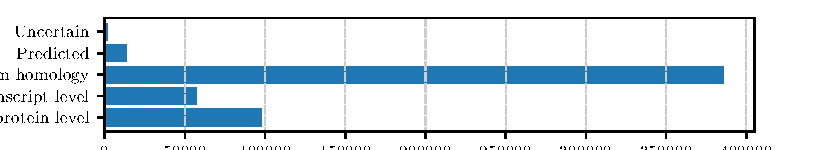
\includegraphics[]{plots/PE.pdf}
  \label{fig:PE}
  \caption{Histogram nivoa pouzdanosti \swissprot proteina}
\end{figure}

% \section{Disprot}
%
% Baza proteinskog neuređenja \en{Database of protein Disorder (DisProt)}
%
% \section{D2P2 i MobiDB}
%
% Baze predviđenog neuređenja proteinskih sekvenci













